\documentclass{article}

\usepackage{tikz}
\usetikzlibrary{automata, positioning}
\begin{document}
\begin{tikzpicture}[shorten >= 1pt, node distance = 2.5cm, on grid, auto]
  \node[state, initial] (0) {0};
  \node[state] (1) [above right=of 0] {1};
  \node[state] (2) [right=of 1] {2};
  \node[state, accepting] (3) [right=of 2] {3};
  \node[state] (4) [below right=of 0] {4};
  \node[state, accepting] (5) [right=of 4] {5};
  \path[->]
    (0) edge node {$\epsilon$} (1)
        edge node {$\epsilon$} (4)
    (1) edge node {i} (2)
    (2) edge node {f} (3)
    (4) edge node {letter} (5)
    (5) edge [loop below] node {letter} (5);
\end{tikzpicture}

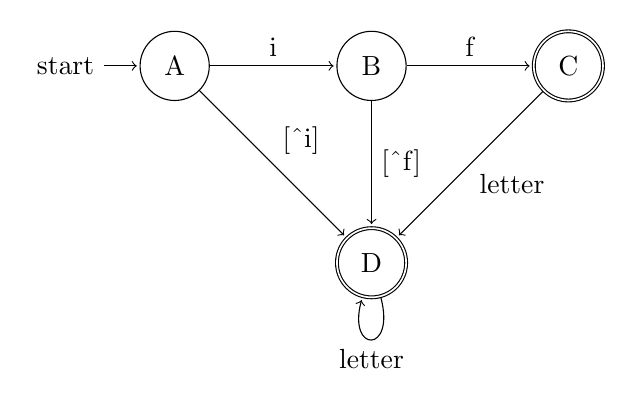
\begin{tikzpicture}[shorten >= 1pt, node distance = 2.5cm, on grid, auto]
  \node[state, initial] (A) {A};
  \node[state] (B) [right =of A] {B};
  \node[state, accepting] (C) [right =of B] {C};
  \node[state, accepting] (D) [below =of B] {D};
  \path[->]
    (A) edge node {i} (B)
        edge node {[\^{}i]} (D)
    (B) edge node {f} (C)
        edge node {[\^{}f]} (D)
    (C) edge node {letter} (D)
    (D) edge [loop below] node {letter} (D);
\end{tikzpicture}
\end{document}
